\documentclass[journal]{vgtc}\usepackage[]{graphicx}\usepackage[]{color}
%% maxwidth is the original width if it is less than linewidth
%% otherwise use linewidth (to make sure the graphics do not exceed the margin)
\makeatletter
\def\maxwidth{ %
  \ifdim\Gin@nat@width>\linewidth
    \linewidth
  \else
    \Gin@nat@width
  \fi
}
\makeatother

\definecolor{fgcolor}{rgb}{0.345, 0.345, 0.345}
\newcommand{\hlnum}[1]{\textcolor[rgb]{0.686,0.059,0.569}{#1}}%
\newcommand{\hlstr}[1]{\textcolor[rgb]{0.192,0.494,0.8}{#1}}%
\newcommand{\hlcom}[1]{\textcolor[rgb]{0.678,0.584,0.686}{\textit{#1}}}%
\newcommand{\hlopt}[1]{\textcolor[rgb]{0,0,0}{#1}}%
\newcommand{\hlstd}[1]{\textcolor[rgb]{0.345,0.345,0.345}{#1}}%
\newcommand{\hlkwa}[1]{\textcolor[rgb]{0.161,0.373,0.58}{\textbf{#1}}}%
\newcommand{\hlkwb}[1]{\textcolor[rgb]{0.69,0.353,0.396}{#1}}%
\newcommand{\hlkwc}[1]{\textcolor[rgb]{0.333,0.667,0.333}{#1}}%
\newcommand{\hlkwd}[1]{\textcolor[rgb]{0.737,0.353,0.396}{\textbf{#1}}}%

\usepackage{framed}
\makeatletter
\newenvironment{kframe}{%
 \def\at@end@of@kframe{}%
 \ifinner\ifhmode%
  \def\at@end@of@kframe{\end{minipage}}%
  \begin{minipage}{\columnwidth}%
 \fi\fi%
 \def\FrameCommand##1{\hskip\@totalleftmargin \hskip-\fboxsep
 \colorbox{shadecolor}{##1}\hskip-\fboxsep
     % There is no \\@totalrightmargin, so:
     \hskip-\linewidth \hskip-\@totalleftmargin \hskip\columnwidth}%
 \MakeFramed {\advance\hsize-\width
   \@totalleftmargin\z@ \linewidth\hsize
   \@setminipage}}%
 {\par\unskip\endMakeFramed%
 \at@end@of@kframe}
\makeatother

\definecolor{shadecolor}{rgb}{.97, .97, .97}
\definecolor{messagecolor}{rgb}{0, 0, 0}
\definecolor{warningcolor}{rgb}{1, 0, 1}
\definecolor{errorcolor}{rgb}{1, 0, 0}
\newenvironment{knitrout}{}{} % an empty environment to be redefined in TeX

\usepackage{alltt}                % final (journal style)
%\documentclass[review,journal]{vgtc}         % review (journal style)
%\documentclass[widereview]{vgtc}             % wide-spaced review
%\documentclass[preprint,journal]{vgtc}       % preprint (journal style)
%\documentclass[electronic,journal]{vgtc}     % electronic version, journal

%% Uncomment one of the lines above depending on where your paper is
%% in the conference process. ``review'' and ``widereview'' are for review
%% submission, ``preprint'' is for pre-publication, and the final version
%% doesn't use a specific qualifier. Further, ``electronic'' includes
%% hyperreferences for more convenient online viewing.

%% Please use one of the ``review'' options in combination with the
%% assigned online id (see below) ONLY if your paper uses a double blind
%% review process. Some conferences, like IEEE Vis and InfoVis, have NOT
%% in the past.

%% Please note that the use of figures other than the optional teaser is not permitted on the first page
%% of the journal version.  Figures should begin on the second page and be
%% in CMYK or Grey scale format, otherwise, colour shifting may occur
%% during the printing process.  Papers submitted with figures other than the optional teaser on the
%% first page will be refused.

%% These three lines bring in essential packages: ``mathptmx'' for Type 1
%% typefaces, ``graphicx'' for inclusion of EPS figures. and ``times''
%% for proper handling of the times font family.

\usepackage{mathptmx}
\usepackage{graphicx}
\usepackage{times}

%% We encourage the use of mathptmx for consistent usage of times font
%% throughout the proceedings. However, if you encounter conflicts
%% with other math-related packages, you may want to disable it.

% declare the path(s) where your graphic files are
\graphicspath{{Figure/}{Images/}{../../Images/}}
% and their extensions so you won't have to specify these with
% every instance of \includegraphics
\DeclareGraphicsExtensions{.pdf,.jpg,.png}

%---------------------------------------------------
\usepackage[cmex10]{amsmath}
\usepackage{amssymb}
\usepackage{color}
\usepackage[dvipsnames,svgnames]{xcolor}
\usepackage{ulem}
\usepackage[section]{placeins}
\usepackage[caption=false,font=footnotesize,labelfont=sf,textfont=sf]{subfig}
\usepackage{sidecap}
\usepackage{multirow}
\usepackage{bbm}
\usepackage{url}
\usepackage{xr}
\usepackage{xr-hyper}

%---------------------------------------------------

%% This turns references into clickable hyperlinks.
\usepackage[bookmarks,backref=section,linkcolor=black]{hyperref} %,colorlinks
\hypersetup{
  pdfauthor = {},
  pdftitle = {},
  pdfsubject = {},
  pdfkeywords = {},
  colorlinks=true,
  linkcolor= black,
  citecolor= black,
  pageanchor=true,
  urlcolor = black,
  plainpages = false,
  linktocpage
}

\externaldocument{TestingVisualAptitude}

%% If you are submitting a paper to a conference for review with a double
%% blind reviewing process, please replace the value ``0'' below with your
%% OnlineID. Otherwise, you may safely leave it at ``0''.
\onlineid{0}

%% declare the category of your paper, only shown in review mode
\vgtccategory{Theory/Model}

%% allow for this line if you want the electronic option to work properly
\vgtcinsertpkg

%% In preprint mode you may define your own headline.
%\preprinttext{To appear in IEEE Transactions on Visualization and Computer Graphics.}

%% Paper title.

\title{Spatial Reasoning and Data Displays}

%% This is how authors are specified in the journal style

%% indicate IEEE Member or Student Member in form indicated below
\author{Susan VanderPlas, and Heike Hofmann, \textit{Member, IEEE}}
\authorfooter{
%% insert punctuation at end of each item
\item
 Susan VanderPlas is a graduate student at Iowa State University. %Email: skoons@iastate.edu.
\item
 Heike Hofmann is a professor at Iowa State University in the Departments of Statistics and Human Computer Interaction. %Email: hofmann@iastate.edu.
}


%other entries to be set up for journal
\shortauthortitle{VanderPlas \MakeLowercase{\textit{et al.}}: Spatial Reasoning and Data Displays}
%\shortauthortitle{Firstauthor \MakeLowercase{\textit{et al.}}: Paper Title}


%% Abstract section.
\abstract{
Graphics convey numerical information very efficiently, but rely on a different set of mental processes than tabular displays. This study examines the demographic characteristics and visual skills associated with perception of graphical lineups. We conclude that lineups are essentially a classification test in a visual domain, and that performance on the lineup protocol is associated with general aptitude, rather than specific tasks such as card rotation and spatial manipulation. We also examine the possibility that specific graphical tasks may be associated with certain visual skills and conclude that more research is necessary to understand which visual skills are required in order to understand certain plot types. 
} % end of abstract

%% Keywords that describe your work. Will show as 'Index Terms' in journal
%% please capitalize first letter and insert punctuation after last keyword
\keywords{Data visualization, Perception, Statistical graphics, Statistical computing.}

%% ACM Computing Classification System (CCS). 
%% See <http://www.acm.org/class/1998/> for details.
%% The ``\CCScat'' command takes four arguments.

\CCScatlist{ % not used in journal version
 \CCScat{H.2.8.c}{Data and knowledge visualization}%
{Database applications}{Database management};
 \CCScat{G.3.n}{Statistical Computing}{Probability and Statistics}{Mathematics of Computing}
}

%% Uncomment below to include a teaser figure.
%    \teaser{
%    \centering
%    \includegraphics[width=16cm]{CypressView}
%    \caption{In the Clouds: Vancouver from Cypress Mountain.}
%   }




%% Uncomment below to disable the manuscript note
%\renewcommand{\manuscriptnotetxt}{}

%% Copyright space is enabled by default as required by guidelines.
%% It is disabled by the 'review' option or via the following command:
% \nocopyrightspace

%%%%%%%%%%%%%%%%%%%%%%%%%%%%%%%%%%%%%%%%%%%%%%%%%%%%%%%%%%%%%%%%
%%%%%%%%%%%%%%%%%%%%%% START OF THE PAPER %%%%%%%%%%%%%%%%%%%%%%
%%%%%%%%%%%%%%%%%%%%%%%%%%%%%%%%%%%%%%%%%%%%%%%%%%%%%%%%%%%%%%%%%
\IfFileExists{upquote.sty}{\usepackage{upquote}}{}
\begin{document}
\setcounter{table}{0}
\renewcommand{\thetable}{A\arabic{table}}
\setcounter{figure}{0}
\renewcommand{\thetable}{A\arabic{figure}}








\appendix
\section{Visuospatial Aptitude Tests}
The Visual Search Task (VST), shown in Figure~\ref{fig:VST}, is used to measure a person's ability to locate a target amid a field of distractors. 
\begin{figure}[htp]\centering
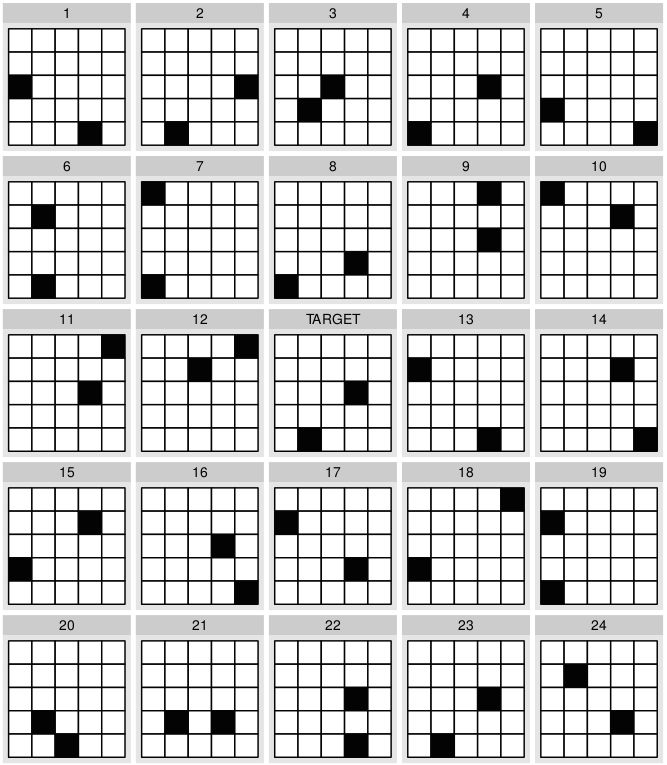
\includegraphics[width=.5\linewidth]{VisualSearch}
\caption[Visual Search Task]{Visual Search Task (VST). Participants are instructed to find the plot numbered 1-24 which matches the plot labeled ``Target". Participants will complete up to 25 of these tasks in 5 minutes.}\label{fig:VST}
\end{figure}

Figure~\ref{fig:tests} shows samples from the figure classification task, the card rotation task, and the paper folding task. All three tasks are part of the Kit of Factor-Referenced Cognitive Tests \cite{ekstrom1976manual}. 
 \begin{figure}[ht]
  \centering
   \subfloat[Figure Classification Task. Participants classify each figure in the second row as belonging to one of the groups above. Participants complete up to 14 of these tasks (each consisting of 8 figures to classify) in 8 minutes.\label{fig:figureclassification}]{%
  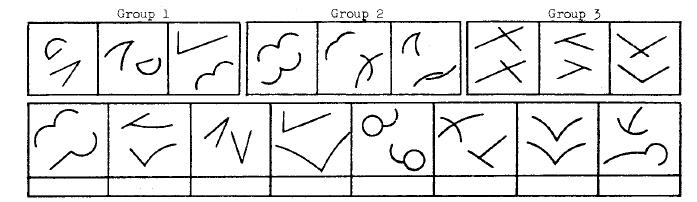
\includegraphics[width=.8\linewidth]{figureclassification}
}
\hfill
    \subfloat[Card Rotation Task. Participants mark each figure on the right hand side as either the same as or different than the figure on the left hand side of the dividing line. Participants complete up to 20 of these tasks (each consisting of 8 figures) in 6 minutes.\label{fig:cardrotation}]{%

\includegraphics[width=.8\linewidth]{cardrotation}
    }
    \hfill
    \subfloat[Paper Folding Task. Participants are instructed to pick the figure matching the sequence of steps shown on the left-hand side. Participants  complete up to 20 of these tasks in 6 minutes.\label{fig:paperfolding}]{%
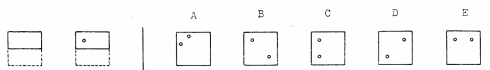
\includegraphics[width=.8\linewidth]{paperfolding}
   }
    \caption{Visuospatial tests}
    \label{fig:tests}
\end{figure}

\section{Scaling Scores}\label{app:ScoreAdj}
To calculate ``scaled" comparison scores between tests which included different numbers of test sections (as shown in Table~\ref{tab:scorecomparison}), we scaled the mean in direct proportion to the number of questions (thus, if there were two sections of equivalent size, and the reference score included only one of those sections, we multiplied the reported mean score by two). The variance calculation is a bit more complicated: In the case described in the main text, where the reference section contained half of the questions, the variance is multiplied by two, causing the standard deviation to be multiplied by approximately 1.41. 

This scaling gets slightly more complicated for scores which have two sub-groups, as with the figure classification test, which separately sumarizes male and female participants' scores. 
To get a single unified score with standard deviation, we completed the following calculations: 
\begin{align}
\mu_{\text{all}} &= (N_F\mu_{F} + N_M\mu_{M})/(N_F + N_M)\\
\sigma_{\text{all}} &= \sqrt{\left(N_F\sigma_F^2 + N_M\sigma_M^2\right)/(N_F + N_M)}.
\end{align}
Here $\mu_F$ and $\mu_M$ are the mean scores for females and males, respectively; $N_F$ and $N_M$ are the number of female and male participants, and $\sigma_F^2$ and $\sigma_M^2$ are the variances in scores for females and males.

Substituting in the provided numbers, we get
\begin{align*}
\mu_{\text{all}} &= \left(323\!\cdot\!114.9\! +\! 294\!\cdot\!120.0\right)/(323\!+\!294) \\
& = 58.7\\
\sigma_{\text{all}} &= \sqrt{\left(323 \cdot 27.8^2 \!+\! 294 \cdot 30^2\right)/(323\!+\!294)} \\
& = 14.4.
\end{align*}

Whenever participants in two studies were not exposed to the same number of questions, the resulting scores are not comparable: both overall scores and their standard deviations are different. We can achieve comparability by scaling the scores accordingly.
For example, in order to account for the fact that ISU students took only part I of two parts to the figure classification test (and thus completed half of the questions), we adjust the transformation as follows:

\begin{eqnarray*}
\mu_{\text{part I}} &= 1/2 \cdot \mu_{\text{all}}\\
\sigma_{\text{part I}} &= 1/\sqrt{2} \cdot \sigma_{\text{all}}
\end{eqnarray*}

\section{Lineup Performance and Demographic Characteristics}\label{app:categoricalresults}
Table~\ref{tab:ttest-demographics} provides the results of a sequence of linear models fit to the lineup data. Each row in the table represents a single model, with one predictor variable (a factor with two or more levels). Due to sample size considerations, multiple testing corrections were not performed; in addition, the independent variables are correlated: in our sample, males are more likely to have completed Calculus 1, but are also more likely to spend time playing video games. As such, a model including two or more of the significant predictor variables shows all included variables to be nonsignificant. To better understand the effects of these variables, a larger study is necessary. 
% latex table generated in R 3.1.2 by xtable 1.7-1 package
% Mon Mar 16 17:53:53 2015
\begin{table}[ht]
\centering
\caption{Participant demographics' impact on lineup score. The table below shows each single demographic variable's association with lineup score. STEM major, completion of Calculus I, time spent playing video games, and gender all show some association with score on statistical lineups. \label{tab:ttest-demographics}} 
\begin{tabular}{lrrrr}
  \hline
Variable & DF & MeanSq & F & p.val \\ 
  \hline
STEM Major & 1 & 401.517 & 14.44 & 0.001 \\ 
  Calculus 1 & 1 & 204.569 & 6.15 & 0.018 \\ 
  Video Game Hours & 3 & 108.847 & 3.44 & 0.028 \\ 
  Sex & 1 & 140.844 & 4.02 & 0.053 \\ 
  Art Skills & 4 & 75.891 & 2.28 & 0.082 \\ 
  Verbal Skills & 3 & 60.220 & 1.68 & 0.191 \\ 
  STEM Research & 1 & 59.670 & 1.60 & 0.214 \\ 
  AutoCAD & 1 & 50.893 & 1.36 & 0.252 \\ 
  Age & 1 & 34.434 & 0.91 & 0.348 \\ 
  Math Skills & 3 & 37.039 & 0.98 & 0.416 \\ 
  Statistics Class & 1 & 9.062 & 0.23 & 0.631 \\ 
   \hline
\end{tabular}
\end{table}


\section{Principal Component Analysis of Visuo-Spatial Tests}\label{app:pca}
\subsection{Importance of principal components in an analysis of the four cognitive tests}\label{app:pca4}

% latex table generated in R 3.1.2 by xtable 1.7-1 package
% Mon Mar 16 17:53:53 2015
\begin{table}[htb]
\centering
\caption{Importance of principal components in an analysis of four tests of spatial ability: figure classification, paper folding, card rotation, and visual search.\label{tab:PCAvariance4}} 
{\footnotesize
\begin{tabular}{rrrrr}
  \hline
 & PC1 & PC2 & PC3 & PC4 \\ 
  \hline
Standard deviation & 1.61 & 0.81 & 0.73 & 0.49 \\ 
  Proportion of Variance & 0.64 & 0.16 & 0.13 & 0.06 \\ 
  Cumulative Proportion & 0.64 & 0.81 & 0.94 & 1.00 \\ 
   \hline
\end{tabular}
}
\end{table}

Table~\ref{tab:PCAvariance4} contains the proportion of the variance in the four cognitive tasks represented by each principal component. PC1 accounts for about 60\% of the variance; Figure~\ref{fig:biplots4} and Table~\ref{tab:PCArotation4} confirm that PC1 is a measure of the similarity between all 4 tests; that is, a participant's general (or visual) aptitude. PC2 differentiates the figure classification test from the visual searching test, while PC3 differentiates these two from the paper folding test. PC4 is not particularly significant (it accounts for 5.9\% of the variance), but it differentiates the card rotation task from the paper folding task.

% latex table generated in R 3.1.2 by xtable 1.7-1 package
% Mon Mar 16 17:53:53 2015
\begin{table}[htb]
\centering
\caption{Rotation matrix for principal component analysis of the four cognitive tests (visual search, paper folding, card rotation, figure classification).\label{tab:PCArotation4}} 
\begin{tabular}{rrrrr}
  \hline
 & PC1 & PC2 & PC3 & PC4 \\ 
  \hline
card.rot & 0.55 & -0.19 & -0.38 & 0.72 \\ 
  fig.class & 0.46 & 0.58 & 0.66 & 0.14 \\ 
  folding & 0.52 & 0.33 & -0.53 & -0.59 \\ 
  vis.search & 0.46 & -0.72 & 0.38 & -0.34 \\ 
   \hline
\end{tabular}
\end{table}


\begin{knitrout}
\definecolor{shadecolor}{rgb}{0.969, 0.969, 0.969}\color{fgcolor}\begin{figure}

{\centering \includegraphics[width=.45\linewidth]{Figure/fig-biplot-pca4-1} 
\includegraphics[width=.45\linewidth]{Figure/fig-biplot-pca4-2} 

}

\caption{Biplots of principal components 1-4 with observations. Principal component analysis was performed on the four cognitive tests used to understand the association between the cognitive skills required for these tests and the skills required for the lineup protocol.  \label{fig:biplots4}}\label{fig:biplot-pca4}
\end{figure}


\end{knitrout}
Figure~\ref{fig:biplots4} shows that the first PC does not differentiate between any of the tasks; it might be best understood as a general aptitude factor. All of the remaining principal components distinguish between the cognitive tasks; 
PC2 and PC3 separate  paper folding from visual search and from the lineup and figure classification tasks, while PC4 and PC5 mainly separate lineups from card rotation and figure classification. This separation allows us to compare the tasks which are similar from among the principal components. 
According to Table~\ref{tab:PCArotation4}, the first three principal components account for 94.1\% of the variance.

\subsection{PCA of Cognitive Tests and Lineups}\label{app:pca5}
PC1 is essentially an average across all tests representing a general ``visual intelligence" factor.
Biplots of the remaining principal components are shown in Figure~\ref{fig:biplots5}. 

\begin{knitrout}
\definecolor{shadecolor}{rgb}{0.969, 0.969, 0.969}\color{fgcolor}\begin{figure}

{\centering \includegraphics[width=.45\linewidth]{Figure/fig-biplots-pca5-1} 
\includegraphics[width=.45\linewidth]{Figure/fig-biplots-pca5-2} 

}

\caption{Biplots of principal components 2-5 with observations. The lineup task appears to be most similar to the figure classification task, based on the plot of PC2 vs. PC3.  \label{fig:biplots5}}\label{fig:biplots-pca5}
\end{figure}


\end{knitrout}

Figure classification is strongly related to lineups (PC2, PC3). Performance on the visual search task  is also related to lineup performance (PC3). These two components highlight the shared demands of the lineup task and the figure classification task: participants must establish categories from provided stimuli and then classify the stimuli accordingly. 

The visual search task is also clearly important to lineup performance: PC3 captures the similarity between the visual search and lineup performance, and aspects of these tasks are negatively correlated with aspects of the paper folding and card rotation tasks within PC3. Paper folding does not seem to be strongly associated with lineup performance outside of the first principal component; card rotation is only positively associated with lineup performance in PC4.

PC4 captures the similarity between lineups and the card rotation task and separates this similarity from the figure classification task; this similarity does not account for much extra variance (10\%), but it may be that only some lineups require spatial rotation skills. PC5 contains only 5\% of the remaining variance, and is thus not of much interest, however, it seems to capture the relationship between the card rotation task and the paper folding and visual search tasks.

\section{Lineup Task Examples}\label{app:lineuptypes}
\subsection{Lineup Set 1}
The experiment in the first lineup section examined the use of boxplots, density plots, histograms, and dotplots to compare two groups which vary in mean and sample size. The experiment was originally designed to explore the use of lineups to test plots of competing design\cite{hofmann2012graphical}. This set of lineups consists of 20 plots selected from the plots used in the full experiment; each set of data is displayed with each of the four plot types. 

\begin{figure}[htbp]\centering
\includegraphics[keepaspectratio=T,width=.8\linewidth]{../../Images/Lineups1/boxplot_1_15_5_4_13}
\caption{Boxplots used to compare the two distributions.}
\end{figure}
\begin{figure}[htbp]\centering
\includegraphics[keepaspectratio=T,width=.8\linewidth]{../../Images/Lineups1/density_1_15_5_4_13}
\caption{Density plots used to compare the two distributions.}
\end{figure}
\begin{figure}[htbp]\centering
\includegraphics[keepaspectratio=T,width=.8\linewidth]{../../Images/Lineups1/dotplot_1_15_5_4_13}
\caption{Dotplots used to compare the two distributions.}
\end{figure}
\begin{figure}[htbp]\centering
\includegraphics[keepaspectratio=T,width=.8\linewidth]{../../Images/Lineups1/histogram_1_15_5_4_13}
\caption{Histograms used to compare the two distributions.}
\end{figure}

\subsection{Lineup Set 2}
The second lineup section also explored two groups of data, this time comparing boxplots, bee swarm boxplots, boxplots with overlaid jittered data, and violin plots. Participants were much more accurate in this experiment than in the experiment described previously, because of the types of plots compared as well as the underlying data distributions. 
\begin{figure}[htbp]\centering
\includegraphics[keepaspectratio=T,width=.8\linewidth]{../../Images/Lineups2/file147f94f6965d7}
\caption{Boxplots.}
\end{figure}
\begin{figure}[htbp]\centering
\includegraphics[keepaspectratio=T,width=.8\linewidth]{../../Images/Lineups2/file147f9e65f0e4}
\caption{Boxplots with jittered points.}
\end{figure}
\begin{figure}[htbp]\centering
\includegraphics[keepaspectratio=T,width=.8\linewidth]{../../Images/Lineups2/file147f9fc58d73}
\caption{Bee swarm boxplots.}
\end{figure}
\begin{figure}[htbp]\centering
\includegraphics[keepaspectratio=T,width=.8\linewidth]{../../Images/Lineups2/file147f93acbb7e4}
\caption{Violin plots.}
\end{figure}

\subsection{Lineup Set 3}
The final lineup section explored QQ-plots from various model simulations, using reference lines, acceptance bands, and rotation to determine which plots allowed participants to most effectively identify violations of normality. Rotated QQ-plots showed lower performance because participants were able to more accurately compare acceptance bands to residuals, and thus could identify that the reference bands were too liberal. As a result, performance was somewhat lower for rotated plots, even though participants were more accurate when comparing the residuals to the reference bands.

\begin{figure}[htbp]\centering
\includegraphics[keepaspectratio=T,width=.8\linewidth]{../../Images/Lineups3/file13876a225d34-single}
\caption{QQ-plot with guide line.}
\end{figure}
\begin{figure}[htbp]\centering
\includegraphics[keepaspectratio=T,width=.8\linewidth]{../../Images/Lineups3/file13877c93dc78-single}
\caption{QQ-plot with acceptance bands.}
\end{figure}
\begin{figure}[htbp]\centering
\includegraphics[keepaspectratio=T,width=.8\linewidth]{../../Images/Lineups3/file13878e5c92f-single}
\caption{QQ-plot rotated 45 degrees.}
\end{figure}


\section{Lineup Plot Types} \label{app:plottypes}
We can also compare participants' performance on specific types of lineup plots compared with their scores on the visual aptitude tests, for instance, accuracy on lineups which require mental rotation may be related to performance on the card rotation task. 



\begin{figure}[ht]\centering
\includegraphics[width=.8\linewidth]{Figure/fig-lineup-types-1}
\caption{Density plots of scaled scores for different types of lineups. For the same experiment (shown by line color), certain types of plots are more difficult to read and are associated with lower participant scores. \label{fig:plottypesdensity}}
\end{figure}

Figure~\ref{fig:plottypesdensity} compares performance on each different type of plot. The $x$ axis shows scaled score, the $y$ axis shows the density of participant scores. As two different lineup tasks utilized boxplots to test different qualities of the distribution of data (outliers vs. difference in medians), different tasks are shown as different colors, so that accuracy on tasks which are shown in blue can be compared to other blue density curves. 

Figure~\ref{fig:scatterplottypes} shows the association between scaled score on each type of lineup and score on the visual reasoning tests. Sample size for each plot type is fairly small - between 5 and 10 plots per individual, so there is low power for systematic inference, but we can establish that the card rotation task is much more significantly associated with the QQ-plots tasks compared to the other tasks. In addition, rotated QQ-plots seem to be much more asssociated with the paper folding task scores than other QQ-plot tasks; this may be because they require more visual manipulation than other QQ-plots.



\begin{figure*}[ht]\centering
\includegraphics[width=\linewidth]{Figure/fig-lineup-types-scores-1}
\caption{Scatterplots of scaled lineup scores by aptitude test scores. There is some indication that different types of lineup tasks may utilize different visual skills; for instance, QQ-plots with confidence bands may require more skill at mental rotation than QQ-plots without the bands. \label{fig:scatterplottypes}}
\end{figure*}

For comparison, the correlation between general lineup score (non-subdivided) and the card rotation test score was 0.505, the correlation between general lineup score and the figure classification test was 0.512, and the correlation between lineup score and the paper folding test was 0.471.While we can compare the correlation strength between tasks, it is clear that the correlation between the score on any single lineup type and a particular visual aptitude score is lower than the overall relationship that we attribute to visual ability. Additional data is imperative to understand the reasoning required for specific types of plots - it is likely that the 5-10 trials per participant presented in each chart in Figure~\ref{fig:scatterplottypes} are simply not sufficient to uncover any specific relationship between reasoning ability and lineup task. 

\bibliographystyle{abbrv}
%%use following if all content of bibtex file should be shown
%\nocite{*}
\bibliography{references}

\end{document}
